\documentclass[12pt]{report}
\usepackage[utf8]{inputenc}
\usepackage{graphicx}
\usepackage{tikz} 
\usepackage{lmodern} 
\usepackage{mathptmx}
\usepackage{helvet}  
\usepackage{csquotes}
\usepackage{hyperref}
\usepackage{palatino}    
\usepackage{tgbonum}   
\usepackage{fancyhdr}
\usepackage{titlesec}
\usepackage{tocloft}
\usepackage{amsmath}     
\usepackage{float}
\usepackage{enumitem}
\usepackage[style=apa, backend=biber]{biblatex}
\usepackage[font=small,labelfont=bf]{caption}
\usepackage[none]{hyphenat}
\usepackage{geometry}
\usepackage[spanish]{babel}
\usepackage{cleveref}


\sloppy
\addbibresource{referencias.bib}


\graphicspath{{figures/}}
\renewcommand{\chaptername}{Capítulo}
\renewcommand{\thesection}{\thechapter.\arabic{section}}
\renewcommand{\thesubsection}{\thesection.\arabic{subsection}}
\renewcommand{\thesection}{\arabic{chapter}.\arabic{section}}

\newfloat{Equation}{htbp}{loe}[chapter]
\floatname{Equation}{}      

\setlength{\cftchapindent}{0pt}    
\setlength{\cftsecindent}{1.5em}  
\setlength{\cftsubsecindent}{3em}  

\setlength{\cftbeforechapskip}{6pt} 
\setlength{\cftbeforesecskip}{4pt}  
\setlength{\cftbeforesubsecskip}{2pt}

\crefname{figure}{Figura}{Figuras}
\Crefname{figure}{Figura}{Figuras}

\fancypagestyle{general}{
  \fancyhf{}
  \fancyhead[L]{
    
\includegraphics[height=2cm]{uaeh.png}
  }
  \fancyfoot[C]{\thepage}
  \fancyhead[C]{
  \raisebox{0.5cm}[0pt][0pt]{
    \vspace{0cm}
    \hspace{1cm}
    \parbox[c]{12cm}{\centering\fontsize{9}{14}\selectfont DESARROLLO DE UN SISTEMA DE RECOMENDACIÓN MUSICAL BASADO EN MÉTODOS DE BÚSQUEDA APROXIMADA DE VECINOS CERCANOS.}}
  }
   \setlength{\headheight}{20pt} 
    \setlength{\headsep}{2.5cm} 
}

\pagestyle{general}

\makeatletter
\let\ps@plain\ps@general
\makeatother

\geometry{top=4cm,bottom=2.5cm,left=3cm,right=3cm}


\title{Sistema de Recomendación Musical basado en la Búsqueda de Vecinos Aproximadamente Más Cercanos.}
\author{ANGEL DAVID FRANCO HERNANDEZ}
\date{August 2025}

\titleformat{\chapter}[display]
  {\normalfont\huge\bfseries}
  {\chaptertitlename\ \thechapter}{20pt}{\Huge}
 \titlespacing*{\chapter}
  {0pt}
  {0ex plus 1ex minus .2ex} 
  {3ex plus .5ex}

\renewcommand{\familydefault}{\sfdefault}
\renewcommand{\figurename}{Figura}
\renewcommand{\thefigure}{\arabic{figure}}
\renewcommand{\listfigurename}{ÍNDICE DE FIGURAS}
\renewcommand{\figureautorefname}{Figura}


\newcommand{\listequationsname}{ÍNDICE DE ECUACIONES}
\newlistof{myequations}{equ}{\listequationsname}

\newcommand{\addequation}[1]{%
  \addcontentsline{equ}{myequations}{#1}%
}
\renewcommand{\theEquation}{Cap. \thechapter, Ec. \arabic{Equation}}


\begin{document}
\thispagestyle{empty}
\begin{titlepage}
      \begin{tikzpicture}[remember picture, overlay]
        \node[anchor = north west, xshift = 1cm, yshift = -1cm] 
            at (current page.north west) 
            {
\includegraphics[width = 3.5cm]{uaeh.png}};
    \end{tikzpicture}

    \begin{tikzpicture}
        [remember picture, overlay]
        \node[anchor=north west, xshift=2cm, yshift=-6cm] 
            at (current page.north west) {
                \parbox{2cm}{
                    \rule{0.1cm}{19cm}%
                    \hspace*{0.2cm}\raisebox{0.5cm}{\rule{0.08cm}{18cm}}
                }
            };
    \end{tikzpicture}

    \hspace*{1.2cm}
    \parbox{15cm}{
        \centering
        \vspace{-2cm}
        \baselineskip=1.5\baselineskip
        {\Large \textsf{\textbf{UNIVERSIDAD AUTÓNOMA DEL ESTADO DE HIDALGO}}}\\[0cm]
        \rule{13.5cm}{2.5pt}\\[-10pt]
        \rule{11cm}{2pt}\\[1.5cm]
    }

    \vspace{-1cm}
    
    \begin{tikzpicture}[remember picture, overlay]
        \node[anchor=north west, xshift=7cm, yshift=-5.5cm] at (current page.north west) {
            {\fontsize{15pt}{18pt}\selectfont
                \textsf{Instituto de Ciencias Básicas e Ingeniería.}
            }
        };
        \node[anchor=north west, xshift=6.3cm, yshift=-6cm] at (current page.north west){
            {\fontsize{15pt}{18pt}\selectfont
                    \textsf{Área Académica de Computación y Electrónica.}}
        };
        \node[anchor=north west, xshift=6.8cm, yshift=-6.7cm] at (current page.north west){
            {\fontsize{15pt}{18pt}\selectfont
                   \textsf{Licenciatura en Ciencias Computacionales.}}
        };
        \node[
            anchor=north west,
            xshift=3.5cm,
            yshift=-9cm,
            text width=16cm,
            align=center
        ] at (current page.north west) {
            \begin{minipage}{\linewidth}
                \centering
                \fontsize{17pt}{25pt}\selectfont
                \textsf{
                    \textbf{"DESARROLLO DE UN SISTEMA DE RECOMENDACIÓN MUSICAL BASADO EN MÉTODOS DE BÚSQUEDA APROXIMADA DE VECINOS CERCANOS".}
                }
            \end{minipage}
        };

        \node[
            anchor=north west,
            xshift=3.5cm,
            yshift=-13cm,
            text width=16cm,
            align=center
        ] at (current page.north west) {
            \begin{minipage}{\linewidth}
                \centering
                \fontsize{13pt}{25pt}\selectfont
                    \textsf{\textbf{TESIS}}\\
                    \textsf{\textbf{QUE PARA OBTENER EL GRADO DE }}\\
                \fontsize{16pt}{25pt}\textsf{\textbf{LICENCIADO EN CIENCIAS COMPUTACIONALES }}\\
                \fontsize{13pt}{25pt}\textsf{\textbf{PRESENTA: }}\\
            \end{minipage}
        };

        \node[
            anchor=north west,
            xshift=3.5cm,
            yshift=-17cm,
            text width=16cm,
            align=center
        ] at (current page.north west) {
            \begin{minipage}{\linewidth}
                \centering
                \fontsize{16pt}{25pt}\selectfont
                    \textsf{ÁNGEL DAVID FRANCO HERNÁNDEZ}
            \end{minipage}
        };

        \node[
            anchor=north west,
            xshift=3.5cm,
            yshift=-19cm,
            text width=16cm,
            align=center
        ] at (current page.north west) {
            \begin{minipage}{\linewidth}
                \centering
                \fontsize{16pt}{25pt}\selectfont
                    \textsf{\textbf{ASESORES:}} \\
                    \textsf{DRA. ANILU FRANCO ARCEGA} \\
                    \textsf{DRA. GUADALUPE CARMONA ARROYO}
            \end{minipage}
        };

         \node[
            anchor=north west,
            xshift=2cm,
            yshift=-26cm,
            text width=16cm,
            align=center
        ] at (current page.north west) {
            \begin{minipage}{\linewidth}
                \fontsize{16pt}{25pt}\selectfont
                    \textsf{Mineral de la Reforma, Hidalgo}
            \end{minipage}
        };

        \node[
            anchor=north west,
            xshift=18cm,
            yshift=-26cm,
            text width=16cm,
            align=center
        ] at (current page.north west) {
            \begin{minipage}{\linewidth}
                \fontsize{16pt}{25pt}\selectfont
                    \textsf{2025}
            \end{minipage}
        };
         
\end{tikzpicture}

\end{titlepage}
\renewcommand{\contentsname}{CONTENIDO }
\renewcommand{\thechapter}{\Roman{chapter}}

\renewcommand{\cftchapfont}{\normalfont}
\renewcommand{\cftsecfont}{\normalfont}
\renewcommand{\cftsubsecfont}{\normalfont}

\renewcommand{\cftchapleader}{\cftdotfill{\cftdotsep}}
\renewcommand{\cftsecleader}{\cftdotfill{\cftdotsep}}
\renewcommand{\cftsubsecleader}{\cftdotfill{\cftdotsep}}
\renewcommand{\cftsubsubsecfont}{\normalfont}  
\renewcommand{\cftsubsubsecleader}{\cftdotfill{\cftdotsep}} 
\renewcommand{\cftsubsubsecpagefont}{\normalfont} 
\setcounter{tocdepth}{3} 

{\raggedright
\tableofcontents
}

\newpage
\pagestyle{general}
\phantomsection
\addcontentsline{toc}{chapter}{ÍNDICE DE FIGURAS}
\listoffigures  

\cleardoublepage
\phantomsection
\addcontentsline{toc}{chapter}{ÍNDICE DE ECUACIONES}
\listofmyequations


\newpage

\chapter*{RESUMEN}
\addcontentsline{toc}{chapter}{RESUMEN}
En los últimos años se ha presentado un avance considerable en las tecnologías y algoritmos de recomendación de contenido digital, principalmente, en uno de los elementos culturales más populares como lo es la música.
Estos algoritmos representan una razón de peso para que un usuario decida permanecer en una plataforma u otra, es por eso que inclusive una mejora minúscula puede significar en un incremento significativo en la satisfacción del usuario.
\\\\
En el presente proyecto se busca potenciar el algoritmo \textit{Voyager} desarrollado por la empresa \textit{Spotify} con el propósito de mejorar los sistemas de recomendación de la plataforma mediante métodos de Búsqueda de Vecinos más Cercanos. Se investigará de manera profunda los fundamentos del algoritmo, sus unidades de medida y la complejidad computacional que genera para ser usado posteriormente en el sistema. 
\\\\
Utilizando esta herramienta como base se desarrollará un sistema web que permita a los usuarios crear una nueva experiencia de escucha denominada como \textit{Viajes Musicales} a través de las herramientas de desarrollo que Spotify hace públicas, usando como fuente de información la \textit{Spotify Web API}, aprovechando sus alcances y evaluando sus limitaciones para obtener la mayor cantidad de información por segundo a través de un algoritmo de búsqueda exhaustiva de canciones.
\\\\
Este algoritmo de búsqueda exhaustiva será planteado por el autor como una capa previa de filtración de música a través de características enteramente \textit{cualitativas}, dando así una muestra signficativa de la cual se pueden obtener recomendaciones más fieles a lo que el usuario le gustaría escuchar.
\\\\
Las aportaciones más importantes de este proyecto se centran en la explicación profunda de los algoritmos de Búsqueda por Vecinos Aproximadamente más Cercanos y por qué son tan eficientes en tareas de recomendación, además de poner en practica el conocimiento en un sistema vinculado a una funcionalidad innovadora, creativa y que mejora la experiencia de escucha musical de los usuarios.

\newpage

\chapter*{ABSTRACT}
\addcontentsline{toc}{chapter}{ABSTRACT}

Nowadays, there has been a considerable improvement in digital recommendation technologies and algorithms, particularly in one of the most popular cultural elements: music. These algorithms represent a compelling reason for a user to choose one platform over another; therefore, even a tiny improvement can result in a significant increase in user satisfaction.
\\\\
This project seeks to enhance the \textit{Voyager} algorithm created by \textit{Spotify}, which is dedicated to improving the platform's recommendation technology using Nearest Neighbor Search methods.
This is done by first thoroughly investigating the algorithm's fundamentals, its units of measurement, and the computational complexity it generates for use in the system.
\\\\
Using this tool as a base, it's been sought to develop a web system that allows users to create a new listening experience named as \textit{Musical Journeys} through the developer tools that Spotify opens to developers using \textit{Spotify Web API} as a source of information, taking advantage of its scope and evaluating its limitations to obtain the greatest amount of information per second through an exhaustive song search algorithm.
\\\\
This exhaustive search algorithm will be proposed by the author as a previous layer of music filtering thorugh entirely qualitative characteristics, thus giving a significant sample from which recommendations more faithful to what the user would like to listen to can be obtained.
\\\\
The most important contributions of this project focus on the in-depth explanation of Approximate Nearest Neighbor Search algorithms and why they are so efficient in recommendation tasks, as well as putting this knowledge into practice in a system linked to innovative and creative functionality that improves users music listening experience

\newpage

\chapter*{INTRODUCCIÓN}
\addcontentsline{toc}{chapter}{INTRODUCCIÓN}

\setlength{\parindent}{0pt}      
\setlength{\parskip}{1em}

Actualmente la música es uno de los productos de entretenimiento con más consumidores en todo el mundo, y su crecimiento ha sido exponencial desde que el formato digital se consolidó en la industria. Plataformas de streaming como Spotify ampliaron el acceso a la música, logrando conectar a sectores que no podían permitirse el formato físico con sus canciones favoritas a un precio considerablemente más bajo. Este cambio transformó la relación de las personas con el arte musical, pasando de ser un lujo a convertirse en un consumo cotidiano.



Spotify ha sido una empresa clave en la digitalización de la música desde la década de 2010, sin embargo, con la consolidación del formato digital se volvió determinante para las empresas del mercado seguir innovando para mantenerse por encima de los competidores.
Por ello, Spotify se ha decantado por invertir en el desarrollo de herramientas que fomenten la preferencia de los usuarios por su plataforma como su favorita para el consumo musical diario.


Durante años los desarrolladores de diferentes empresas han invertido tiempo y recursos en la investigación de métodos eficientes de recomendación para sistemas con información masiva, sin embargo, se han encontrado con dificultades crecientes relacionadas al consumo de recursos computacionales y al tiempo estimado de respuesta que, al hablar de empresas multinacionales con millones de usuarios, debe ser signficativamente rápido.


Como resultado de estos esfuerzos, el equipo de desarrolladores de Spotify ha diseñado diversas herramientas que mejoran la recomendación de música basadas en algoritmos que emplean técnicas de minería de datos y machine learning, logrando minimizar los obstaculos computacionales inherentes al problema a resolver.

No obstante, a pesar de que Spotify ha desarrollado algoritmos eficientes de búsqueda de recomendaciones, persisten áreas de oportunidad a ser tomadas en cuenta. En este proyecto se identifica una de ellas aún no abordada por la plataforma principal ni por herramientas externas y se propone un sistema desarrollado en el entorno web que soluciona esta problemática a través de una propuesta innovadora y creativa, complementando las investigaciones actuales que Spotify ha logrado en los últimos años.

\newpage
\thispagestyle{plain}
\vspace*{0.2cm}

\section*{PLANTEAMIENTO DEL PROBLEMA}
\addcontentsline{toc}{section}{PLANTEAMIENTO DEL PROBLEMA}

En la actualidad, el uso de la plataforma de Spotify le permite al usuario establecer sesiones de escucha de las siguientes maneras:

\begin{enumerate}
    \item \textbf{Elegir manualmente las canciones a escuchar:} Esto implica elegir cada una de las canciones que serán reproducidas en el espacio de tiempo que el usuario decida siguiendo un orden establecido. Este caso de uso se ha exponenciado con el uso de \textit{Listas de Reproducción} \footnote{\textbf{Lista de Reproducción: } Colección ordenada de canciones que se pueden reproducir de forma consecutiva. Se almacenan para ser usadas en el futuro.}.

    \item \textbf{Elegir una canción base como la fuente de recomendaciones:} Sucede cuando el usuario elige una canción que no pertenece a una Lista de Reproducción previamente almacenada, provocando que Spotify ejecute el algoritmo de recomendación tomando de referencia la canción elegida por el usuario. Además, la \textit{Canción base} también es usada cuando la Lista de Reproducción termina de reproducirse totalmente, generando el mismo comportamiento.
\end{enumerate}

Esto indica una problemática emergente: El usuario tiene poco o nulo control de las recomendaciones que la plataforma brinda, teniendo que elegir una sesión de escucha de forma manual o cambiando la \textit{canción base} constantemente. Como resultado, en largas sesiones de escucha, el usuario no sabrá qué canciones elegir o, en el caso de usar el algoritmo de recomendación, es probable que se aburra de escuchar temas similares por largos periodos de tiempo.

Esta situación refleja un área de oportunidad en la que el usuario pueda mantener un control más fino sobre el funcionamiento del algoritmo de recomendación, permitiendo así el diseño de sesiones de escucha prolongadas con mayor diversidad. De esta manera, se plantea la necesidad de explorar métodos alternativos de recomendación que complementen los enfoques actuales empleados por Spotify.

\newpage
\thispagestyle{plain}
\vspace*{0.2cm}

\section*{PROPUESTA DE SOLUCIÓN}
\addcontentsline{toc}{section}{PROPUESTA DE SOLUCIÓN}

En el presente proyecto se plantea una solución creativa e innovadora que le brinda al usuario una capa extra de personalización y control del algoritmo de recomendación a través del concepto de \textit{Viajes Musicales}.

En esta tesis se introducen un conjunto de conceptos que servirán como base para el desarrollo del sistema. En particular, se propone el concepto de \textit{Viaje Musical}, que es definido como una sesión de escucha formada por un conjunto de canciones, de las cuales el usuario solo se preocupará por las que se denominan \textit{estaciones}. El concepto de estaciones es definido como  aquellas canciones que el usuario elige y que representan la guía que tomarán los algoritmos de recomendación para forjar un camino coherente entre las diferentes estaciones, creando así un viaje musical guiado por el usuario pero enriquecido por el sistema.

Con el objetivo de alcanzar dicho nivel de interacción se propone desarrollar un sistema web en donde el usuario pueda vincular su cuenta de Spotify, elegir su viaje musical y vincular la lista de canciones resultante a su cuenta de forma automática, simplificando al máximo la experiencia del usuario para lograr una herramienta cotidiana y fácil de usar.

Por esta razón se busca desarrollar un algoritmo de recomendación que se inspire en los desarrollados por la plataforma aprovechando los recursos públicos que la empresa facilita como la \textit{Spotify Web API} o el algoritmo de recomendación \textit{Voyager}.

En conclusión, la propuesta no solo busca mejorar las recomendaciones existentes, sino ofrecer al usuario una experiencia activa, flexible y narrativa en su consumo musical. De esta manera, los viajes musicales representan un puente entre el control total del usuario y la automatización de los algoritmos, creando una experiencia de escucha dinámica y personalizada que actualmente no existe en la plataforma.

\newpage
\thispagestyle{plain}
\vspace*{0.2cm}

\section*{JUSTIFICACIÓN}
\addcontentsline{toc}{section}{JUSTIFICACIÓN}



En la actualidad, los algoritmos de recomendación representan un elemento clave en la competitividad de los sistemas de entretenimiento digital, ya que permiten ofrecer experiencias personalizadas y mantener la fidelidad de los usuarios. Comprender a fondo las aportaciones previas en este ámbito es esencial para aprovecharlas de manera óptima y generar mejoras que impacten de forma directa en la satisfacción de los usuarios.

Dentro de las técnicas más utilizadas, los algoritmos de Búsqueda de Vecinos Aproximadamente más Cercanos constituyen una herramienta con múltiples aplicaciones, incluyendo el ámbito musical. En particular, el algoritmo \textit{Voyager} fue desarrollado con el objetivo de simplificar la implementación de este tipo de metodologías. Sin embargo, su uso resulta limitado cuando no se entiende a profundidad su funcionamiento, lo cual puede derivar en discrepancias entre los filtros aplicados y los resultados obtenidos. Por esta razón, este proyecto se centra en explicar de manera detallada tanto los fundamentos de la Búsqueda de Vecinos Cercanos como la lógica interna de \textit{Voyager}, con el fin de optimizar su aprovechamiento en sistemas de recomendación.

Además, se propone una nueva capa de \textit{Filtrado por características Cualitativas} que \textit{Voyager} por naturaleza no es capaz de soportar, añadiendo así una innovación técnica enfocada en búsquedas heurísticas adicionales previo al paso de recomendación.

Ambas aportaciones desarrolladas en el contexto musical le permitirán a los usuarios vincularse de forma diferente con las sesiones de música, dándoles un control adicional sobre un algoritmo que, actualmente, está totalmente cerrado al funcionamiento técnico. Este proyecto propone conectar al usuario con su algoritmo y explotar esa interacción de forma innovadora.

Adicionalmente, la implementación de un sistema basado en esta metodología no solo contribuye a fortalecer la investigación en el área, sino que también ofrece a nuevos desarrolladores una base sólida y bien documentada para el diseño de arquitecturas emergentes. De esta manera, el presente trabajo no solo atiende una necesidad técnica, sino que también abre la posibilidad de inspirar nuevas propuestas en el campo de los sistemas de recomendación de cualquier ámbito.


\newpage
\thispagestyle{plain}
\vspace*{0.1cm}

\section*{OBJETIVO GENERAL}
\addcontentsline{toc}{section}{OBJETIVO GENERAL}


Desarrollar un sistema web de recomendación musical  que le permita al usuario generar sesiones de escucha completas a partir de un conjunto representativo de canciones que servirá como base, las cuales permitirán que el sistema complete la lista mediante recomendaciones personalizadas, implementando algoritmos de búsqueda inteligentes.


\subsection*{OBJETIVOS ESPECÍFICOS}
\addcontentsline{toc}{subsection}{OBJETIVOS ESPECÍFICOS}

\begin{enumerate}
    \item Investigar la metodología de Búsqueda de Vecinos Aproximadamente más Cercanos para identificar las deficiencias de los métodos actuales en el entorno de sistemas de recomendación revisando literatura científica y técnica relevante.
    
     \item Implementar el algoritmo \textit{Voyager} con el fin de resolver de forma eficiente el problema de recomendación abordado, configurando sus propiedades de manera justificada y bien documentada.

    \item Crear un algoritmo de \textit{Generación de Muestra Significativa} añadiendo una capa de filtrado \textit{Cualitativo} que ayude con el problema de recomendación musical. 
    
    \item Desarrollar un sistema web dividido en capas que logre implementar los algoritmos de recomendación planteados y, además, obtenga información de la \textit{Spotify Web API} que será usada para las recomendaciones. 
    
    \item Utilizar la \textit{Spotify Web API} para facilitar al usuario la posibilidad de vincular su cuenta de Spotify de forma segura y alineada a los estándares de la plataforma.
    
    \item Desarrollar una interface de usuario llamativa que muestre el concepto de \textit{Viaje Musical} y permita obtener una sesión de escucha coherente basada en \textit{Estaciones} haciendo uso de tecnología web.

\end{enumerate}

\newpage

\chapter{MARCO TEÓRICO }

En el presente capítulo se abordarán los temas más importantes que servirán como base para el desarrollo del proyecto. En particular, se explicarán los fundamentos de los sistemas de recomendación, haciendo enfasis en los diferentes enfoques y técnicas más utilizadas en este campo. Además, se presentará una revisión detallada de los algoritmos de Búsqueda de Vecinos, cómo funcionan y las métricas que utilizan con el fin de entender a profundidad los algoritmos actuales como \textit{Voyager}, que será explicado en detalle al final del capítulo.

\section{FUNDAMENTOS DE LOS SISTEMAS DE RECOMENDACIÓN }

Los sistemas de recomendación son \textbf{agentes de información personalizada} que brindan sugerencias de elementos que \textit{podrían} ser útiles para un usuario.  Los resultados dados por un sistema de recomendación se denominan \textbf{Recomendaciones} que representan una opción valiosa que podría ser del interés de una persona o usuario.

\subsection[CONCEPTOS BÁSICOS]{CONCEPTOS BÁSICOS DE LOS SISTEMAS DE RECOMENDACIÓN }


Los Sistemas de Recomendación se fundamentan mediante entidades que aportan información desde diferentes medios:

\begin{itemize}
    \item \textbf{Usuario: } La entidad a la que se le hacen llegar las recomendaciones es denominada como \textit{usuario}. 
    \item \textbf{Items: } Es una pieza de información que refiere a un objeto tangible o digital que el sistema de recomendación sugerirá al usuario en una interacción a través de la Web, email o mensajes de texto \parencite{Kotkov2020Serendipity}.
    \item \textbf{Fuente de Conocimiento: } Determina qué técnica será usada para definir el medio de información y determinar el conocimiento necesario para brindar sugerencias relevantes.
\end{itemize}

El principio básico que fundamenta a los algoritmos de recomendación es la dependencia significativa que existe entre un \textit{usuario} y los \textit{items} con los que interactúa.

\subsection[OBJETIVOS GENERALES]{OBJETIVOS DE UN SISTEMA DE RECOMENDACIÓN: }

Según \parencite{Aggarwal2016} más allá de los objetivos mercadológicos que se le atribuyen a los sistemas de recomendación enfocados en mejorar el rendimiento económico de una plataforma, se pueden definir objetivos técnicos y operacionales que mejoran el rendimiento de un sistema en éste ámbito.

\begin{itemize}
    \item \textbf{Relevancia: }Un sistema de recomendación siempre debe brindar sugerencias relevantes para el usuario.
    \item \textbf{Novedad: }  Las recomendaciones suelen ser más útiles cuando sugieren elementos que el usuario no ha visto antes. Además, recomendar los objetos más populares puede conducir a reducir la diversidad del consumo.
    \item \textbf{Sorpresa: } No basta con que los objetos de recomendación sean nuevos para el usuario, sino que también deben sorprenderlo, dándole la sensación de un \textit{descubrimiento inesperado.}
    
    \item \textbf{Diversidad de Recomendaciones: } La lista de sugerencias obtenidas deben ser suficientemente diferentes entre sí para no aburrir al usuario, sin embargo, la diversidad de \textit{items} no debe alejarse demasiado de sus preferencias.
   \enquote{\textit{La diversidad tiene el beneficio de asegurar que el usuario no se aburre de constantes recomendaciones de items similares. }} [\cite{Aggarwal2016}]
\end{itemize}

\newpage

Existen dos versiones diferentes que definen los resultados esperados de un Sistema de Recomendación, ambos buscan resolver el problema de encontrar items relevantes para los usuarios mediante modelos distintos:


\begin{enumerate}
    \item \textbf{Versión de Predicción: } Se basa en predecir la calificación que el usuario daría a un item. Se asume que existe un conjunto de Datos de Entrenamiento que indica las preferencias del usuario.
    \item \textbf{Versión de Top - $k$: } Este enfoque argumenta que muchos de los sistemas no necesitan conocer la calificación estimada del usuario, por el contrario, solo necesitan saber qué recomendar sin necesidad de estimar una calificación exacta. Esto se suele hacer mediante un Top - $k$ elementos que probablemente le gusten al usuario.
\end{enumerate}

\subsection{PRINCIPALES ENFOQUES DE RECOMENDACIÓN }
Para que un sistema de recomendación logre cumplir los objetivos básicos esperados se necesita establecer de forma clara cuál será el filtro para sugerir items al usuario eligiendo diferentes enfoques que se adapten a los resultados que se buscan obtener.

Basándose en \parencite{ISINKAYE2015261} existen diferentes filtros de recomendación principales, sin embargo, se muestran los más relevantes para el presente proyecto:

\subsubsection[BASADO EN CONTENIDO]{ENFOQUE BASADO EN CONTENIDO }
Es una técnica de sistema de recomendación que se centra en el análisis de atributos de cada item para generar predicciones sobre las preferencias del usuario. Se apoya de valoraciones previamente vinculadas a un perfil que permiten identificar características clave de los objetos que el usuario ha calificado, principalmente de aquellos que cuentan con una valoración positiva.  Por esta razón, la eficacia de este enfoque se basa en la cantidad de información disponible de los items.

Los algoritmos que implementan esta técnica suelen basarse en modelos de análisis estadístico y de \textit{Machine Learning.}

\newpage

\textbf{VENTAJAS }
\begin{itemize}

    \item \textbf{Capacidad recomendar items nuevos: } Este enfoque permite sugerir elementos que aún no han sido evaluados por los usuarios gracias a la información contenida en sus \textit{metadatos} \footnote{\textbf{Metadatos: } Atributos que describen, proveen contexto, indican la calidad, o documentan las características de un objeto. \parencite{Greenberg09092005}}.
    \item \textbf{Alta adaptabilidad: } Se adapta a los cambios de preferencia del usuario en un lapso corto de tiempo.

    \item \textbf{Independencia entre usuarios: } Los usuarios reciben recomendaciones sin la necesidad de compartir su información con externos, priorizando la privacidad y seguridad de los datos.
    
\end{itemize}

\textbf{DESVENTAJAS }
\begin{itemize}

    \item \textbf{Dependencia en la profundidad de la información: } Los motores de recomendación basados en esta técnica son dependientes de los metadatos vinculados a los items. Por lo tanto, requieren que los elementos sean profundamente descritos por sus atributos. Esto es definido como \textbf{\textit{Análisis limitado al contenido}}.
    
    \item \textbf{Falta de Diversidad: } Es probable que las sugerencias sufran de \textit{sobre-especialización} o, en otras palabras, que carezcan de diversidad debido a que los usuarios están restringidos a obtener recomendaciones similares a los items asociados a sus perfiles.
\end{itemize}

\subsubsection[COLABORATIVO]{ENFOQUE COLABORATIVO}

A diferencia del enfoque basado en contenido, que se centra en los atributos de los items, el enfoque colaborativo se centra en las similitudes entre lo usuarios para generar recomendaciones.

Este enfoque funciona construyendo una base de datos descrita por una matríz \textit{usuarios - items} que representa la preferencia de un conjunto de usuarios por un item particular. Esto significa que vincula a diferentes perfiles con preferencias e intereses similares para guiar las recomendaciones, formando así un grupo  de perfiles que comparten intereses denominado \textit{Vecindario}. 


Por lo tanto, un usuario recibe recomendaciones de contenido que no ha evaluado pero que otros usuarios dentro de su \textit{Vecindario} han calificado de forma positiva. Los resultados que se pueden obtener a través de este enfoque son los siguientes:

\begin{itemize}
    \item \textbf{Predicciones: } Es un valor numérico que expresa un puntaje del elemento $j$ para el usuario $i$, esta predicción se representa con la notación $R_{i,j}$.
    \item \textbf{Rankings: } Es una lista de los Top - $N$ elementos que al usuario le podrían gustar más.
\end{itemize}

\begin{figure}[h!]
    \centering
    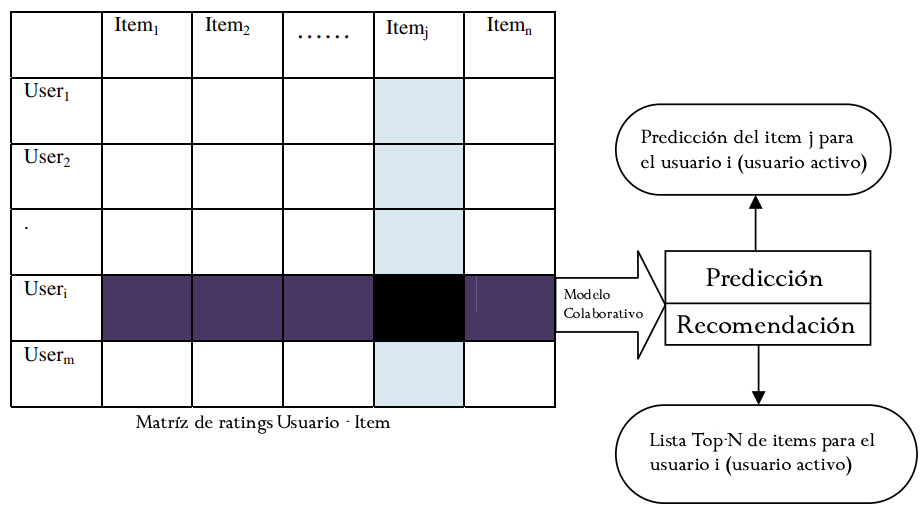
\includegraphics[width=0.7\linewidth]{FiltroBasadoenContenido.png}
    \caption{Ejemplo del Filtro Basado en Colaboración \parencite{ISINKAYE2015261}.}
    \label{fig:FiltroColaborativo}
\end{figure}

En la figura \ref{fig:FiltroColaborativo} se muestra un ejemplo de funcionamiento del enfoque colaborativo. Se puede observar que la matríz está compuesta por filas que representan a los usuarios de un mismo \textit{Vecindario}, y por columnas que representan a los \textit{items}. Las intersecciones mostradas de color morado representan la calificación que el usuario ha dado a elementos previos, y la intersección diferenciada de color negro expresa una predicción basada en las calificaciones que los vecinos han asignado a ese item.
El diagrama remarca la distinción entre \textit{Predicción} y la \textit{Recomendación} dado que, en el caso de la predicción,  la intersección representada en color negro representa el valor $R_{i,j}$, y en el caso de la recomendación representa un \textit{item} dentro de los Top - $N$ items del usuario actual.

\newpage

\textbf{VENTAJAS}

Este enfoque tiene ventajas fuertemente diferenciadas respecto al enfoque basado en contenido, algunos de sus puntos fuertes son los siguientes:

\begin{itemize}
    \item \textbf{Independencia al Contenido: } Los algoritmos colaborativos pueden funcionar de forma efectiva en dominios en los cuales no existe diversidad de información (o metadatos) para describir los items.
    \item \textbf{Recomendaciones basadas en Serendipia \footnote{\textbf{Serendipia en Sistemas de Recomendación: } \textit{Items} que son relevantes pero inesperados para el usuario. \textit{Items} que son nuevos e inesperados. \parencite{Kotkov2020Serendipity}} }: Significa que tiene la capacidad de recomendar elementos que son aparentemente ajenos a las preferencias del usuario, pero que para sus \textit{vecinos} son relevantes, conectando al usuario con contenido nuevo.
\end{itemize}

\textbf{DESVENTAJAS}

\begin{itemize}
    \item \textbf{Problema de \textit{Inicio Frío}}: Se refiere a la situación en donde el Sistema de Recomendación no tiene información adecuada acerca del usuario o acerca del item para hacer predicciones relevantes \parencite{Burke2007}. Este problema es crucial ya que este enfoque se vuelve dependiente de conocer con el tiempo las preferencias del usuario que, inicialmente, son desconocidas.

    \item \textbf{Problema del \textit{Esparcimiento de Datos}}: Otro de los puntos de los que depende el enfoque colaborativo es en las calificaciones hechas por los usuarios, causando la necesidad de que existan previas valoraciones para los items, de lo contrario, se generan recomendaciones poco relevantes.
    
    \item \textbf{Escalabilidad}: Un problema bastante común en los algoritmos de recomendación con enfoque colaborativo es la escalabilidad. Cuando la cantidad de usuarios e items crecen rápidamente, la complejidad computacional crece de forma lineal en relacion a estos dos aspectos, dando un costo computacional representado por la siguiente fórmula: $O(items \ \cdot \ usuarios)$\footnote{\textbf{Notación \textit{BIG O}:}  Es un estándar que describe el orden de crecimiento de un algoritmo en función del tamaño del problema. En el presente documento se usará para expresar la complejidad computacional de los algoritmos descritos.}. Es importante mencionar que un algoritmo lineal no logra ser eficaz cuando la cantidad de información es masiva.

    \newpage

    \item \textbf{\textit{Sinónimos: }} Se refiere a la situación en la que items muy similares aparecen registrados con diferentes nombres o identificadores \parencite{ISINKAYE2015261}. Los sistemas de colaboración no reconocen automáticamente que se trata de equivalencias; por ejemplo, \textit{item 1: Álbum Let It Be - The Beatles}, \textit{item 2: Álbum Let It Be (Remasterizado) - The Beatles}. En este caso, el sistema podría tratarlos como elementos completamente diferentes, a pesar de estar estrechamente relacionados.
\end{itemize}

\textbf{ENFOQUE HÍBRIDO}

A pesar de que los enfoques de recomendación basados en contenido y colaborativos son eficaces en escenarios particulares, sus desventajas inherentes limitan su escalabilidad en plataformas de uso masivo.  El enfoque híbrido busca solventar las desventajas de cada enfoque combinando diferentes técnicas de recomendación con el objetivo de evitar las limitaciones y problemas que los enfoques puros pueden enfrentar.

Los sistemas de recomendación híbridos están fuertemente relacionados al campo del \textit{Análisis de Conjuntos (Ensemble Analysis)} en los cuales se combina el poder de multiples tipos de algoritmos basados en \textit{Machine Learning} para crear modelos más robustos \parencite{Aggarwal2016}.  

\textbf{TÍPOS DE ENFOQUES HÍBRIDOS}
\begin{itemize}
    \item \textbf{Enfoque Híbrido basado en Pesos: } Este enfoque combina los resultados de diferentes enfoques de recomendación para crear una lista de recomendaciones que integran las calificaciones de cada técnica mediante una fórmula lineal. Inicialmente todas las técnicas usadas inician con un peso igualado que se modifica a través de la evaluación del usuario.
    \item \textbf{Enfoque Híbrido por Conmutación: } Este enfoque se basa en una heurística definida que selecciona la mejor técnica de recomendación adaptada al momento. Por ejemplo, si se necesita de un algoritmo de recomendación para un usuario nuevo, se puede identificar que usar el enfoque colaborativo no es una buena opción debido al \textit{Inicio Frío}, por lo tanto, se elige el enfoque basado en contenido. El beneficio de esta estrategia es que el sistema es sensible a las fortalezas y debilidades de sus enfoques de recomendación \parencite{ISINKAYE2015261}. 

    Sin embargo, esta conmutación de enfoques tiene una desventaja inherente debido al costo computacional que requiere el cambiar de métodos constantemente, principalmente por la diferencia de criterios y parámetros de información que cada enfoque requiere.

    \item \textbf{Enfoque Híbrido Combinado: } Este enfoque combina los resultados de diferentes algoritmos de recomendación, ejecutándolos en paralelo para generar una lista única de recomendaciones. El beneficio principal de esta estrategia es que el rendimiento local de un enfoque específico no suele afectar de manera significativa al rendimiento global del sistema, resultando en una mayor robustez.
    
\end{itemize}

\section[EVALUACIÓN DE UN SISTEMA DE RECOMENDACIÓN]{PARADIGMAS Y MÉTRICAS DE EVALUACIÓN PARA UN SISTEMA DE RECOMENDACIÓN: }

Los Sistemas de Recomendación deben desarrollarse mediante un enfoque alineado con los objetivos esperados respecto a la interacción con los usuarios. Estos objetivos principales han sido estudiados y seccionados en paradigmas de evaluación, sin embargo, basándose en la investigación de \parencite{Aggarwal2016} se pueden definir también métricas de evaluación generales para calificar el desempeño de un sistema de recomendación. En esta sección se mencionarán generalidades de los paradigmas de evaluación y se hará un enfasis en las métricas generales.

\subsection{PARADIGMAS DE EVALUACIÓN: }

Existen tres paradigmas de evaluación principales dirigidos a los sistemas de recomendación, donde las principales diferencias se centran en cómo los usuarios interactúan con las métricas de evaluación.

\begin{enumerate}

    \item \textbf{Usuarios de Estudio: } Este paradigma se centra en invitar a los usuarios a un proceso de evaluación para interactuar con el sistema y evaluar su desempeño en contextos específicos. Por lo tanto, las mediciones se obtienen de los comentarios de los usuarios y de las observaciones de interacción obtenidas  por el sistema. 
    Esta información se usa para entender cuáles fueron las preferencias del usuario, qué le gustó y qué no le gustó.

    La principal ventaja de este paradigma es que los usuarios dan permisos explícitos para usar su información en función de la evaluación del sistema, sin embargo, las desventajas más significativas radican en los cambios inconscientes del usuario al estar en un escenario de evaluación y en la poca escalabilidad del método. 
    Es probable que no todos los usuarios estén de acuerdo en participar en un escenario de evaluación, y aquellos que lo hagan podrían no tener preferencias significativas alineadas con la mayoría de la población o, en resumen, se podrían obtener resultados específicos pero no representativos.

    Las desventajas mencionadas ocasionan que este paradigma sea usado sólo en entornos académicos o de proyectos que no sean de gran escala.
    
    \item{\textbf{Evaluación \textit{Online}}}: Este paradigma de igual manera depende de la interacción del usuario pero en un entorno de uso real, lo que fomenta resultados más naturales debido a que ahora se interactúa con el sistema en una situación cotidiana. Una de las fortalezas más importantes de este paradigma es que funciona combinando diferentes \textit{enfoques de los sistemas de recomendación} para evaluar cuál se comporta mejor en un escenario en particular. 
    Para comparar el rendimiento de diferentes enfoques se usan métricas concretas como la tasa de conversión, CTR, tiempo de interacción, etc... Estos métodos son también conocidos como \textit{Pruebas} $A / B$ y miden el impacto directo del sistema de recomendación hacia el usuario. 
 
    \textit{"La idea básica es similar a un apostador (el sistema de recomendación) que debe elegir una máquina tragamonedas (diferentes enfoques de recomendación) en un casino. El apostador sospecha que una de las tragamonedas tiene un porcentaje de retorno más alto (tasa de conversión, CTR, etc...) que las demás. Por lo tanto,  el apostador juega con cada tragamonedas de forma individual para observar el porcentaje de retorno de cada máquina. De forma codiciosa el apostador selecciona solo aquella tragamonedas que tenga un rendimiento mas efectivo respecto a las demás"} \parencite{Aggarwal2016}.

    Una de las ventajas más grandes de este paradigma es que permite medir de forma algorítmica el rendimiendo de diferentes \textit{enfoques de recomendación} para obtener el mejor rendimiento posible a través de la interacción directa del usuario. Sin embargo, la principal desventaja es que estos sistemas no pueden ser implementados de forma realista a menos de que se tenga una cantidad masiva de usuarios, haciendo que sea muy complejo de usar en las fases iniciales del sistema.

    La necesidad de contar con una cantidad masiva de usuarios surge de los métodos de \textit{Pruebas} $A / B$ que agrupa a los usuarios en muestras aleatorias a las que se les aplican diferentes algoritmos de recomendación y se mide la satisfacción del usuario mediante diferentes métricas. Para que las mediciones retornen resultados relevantes cada grupo debe contar con un gran número de usuarios.

    \item \textbf{Evaluación \textit{Offline} con \textit{Datasets}\footnote{\textbf{Dataset: } Es una colección de elementos relacionados organizados y con un formato para cumplir un propósito particular \parencite{chapman-2019}.} Históricos: } En la evaluación Offline se trabaja con datos históricos como, por ejemplo, las calificaciones de un usuario a items del sistema. La principal ventaja de trabajar con \textit{Datasets} de información es que se tiene un conjunto grande de información previamente recopilada y no se tiene la necesidad realizar un seguimiento a miles de usuarios activos para evaluar el sistema. Una vez que un \textit{Dataset} ha sido recolectado se puede usar como principal punto de referencia para comparar diferentes algoritmos.
    
    Además, se pueden utilizar diversos datasets que favorezcan la \textit{generalidad} del Sistema de Recomendación.

    Sin embargo, la principal desventaja de la \textit{Evaluación Offline} es que no logra predecir cómo reaccionará el usuario al sistema en el futuro.
    A pesar de estas áreas de oportunidad, éste paradigma sigue siendo uno de los más usados y aceptados para la evaluación de sistemas de recomendación, esto se debe a que las estadísticas que se pueden obtener de estos métodos son robustas, confiables y fáciles de entender.

\end{enumerate}

\subsection{MÉTRICAS GENERALES DE EVALUACIÓN: }

Además de los paradigmas de evaluación que definen metodologías específicas para realizar pruebas a los usuarios, existen métricas cuantificables que añaden una capa extra de complejidad y robustez a los sistemas de recomendación. Estas metricas cumplen la función de asegurar resultados satisfactorios para el usuario mediante características cuantificables y subjetivas, entendiendo que el gusto y las preferencias pueden ser complejas de representar mediante mediciones numéricas.

    \subsubsection{EXACTITUD}

    La exactitud es una de las métricas fundamentales con las que se evalúan los sistemas de recomendación. Se basan en \textit{ratings} que se definen como \textit{"cantidades numéricas que deben ser estimadas" } \parencite{Aggarwal2016}. Sin embargo, como ha sido mencionado anteriormente, algunos enfoques de recomendación no se centran en predecir calificaciones sino que reunen el top-$k$ de los \textit{items} más favorables. 

    \newpage

    La medición por exactitud tiene diversos componentes que aseguran su efectividad:

    \begin{itemize}
        \item \textbf{\textit{Métricas de Efectividad: }} Las Métricas de Efectividad son usadas para evaluar tanto la efectividad de predicción para estimar la calificación de un usuario específico respecto a un item o la efectividad del top - $k$ sugerido por el sistema de recomendación \parencite{Aggarwal2016}.
        
        Existen dos métodos diferentes para medir la efectividad de las predicciones y de los top - $k$:

        \begin{itemize}[label=$\diamond$]
            \item \textbf{\emph{Efectividad de Predicción: }} Se centra en medir el \textit{Error Específico de Entrada} \footnote{\textbf{Error Específico de Entrada: } Diferencia entre la calificación que el sistema de recomendación predice y la calificación real que el usuario dio.} que se define mediante la siguiente fórmula:
            \begin{equation}
                \Large e_{uj} \ = \ \hat{r}_{uj} \ - \ r_{uj}
            \addequation{Definición de Error Específico de Entrada}
            \end{equation}

            \begin{description}
                \item[\textbf{Donde: }] 
                \item[$u$] representa al usuario.
                \item[$j$] representa al item.
                \item[$\hat{r}_{uj}$] representa la predicción de calificación.
                \item[$r_{uj}$] representa la calificación real del usuario. 
            \end{description}

            Este cálculo de $e_{uj}$ puede ser aprovechado de diferentes maneras para hacer un calculo sobre el conjunto de errores de predicción $E$ y los rankings vinculados a cada $e \in E$ \footnote{\textbf{Pertenencia $\in$}: Éste símbolo indica que un elemento cualquiera $u$ \textit{pertenece} a un conjunto $R$, por lo tanto $u \in R$}.

            Para sintetizar, se dice que el conjunto $E$ es definido por: 

            \begin{equation}
                E \ =  \{ \  e_{uj} \ |  \ (u,j) \in D \ \}
                \addequation{Definición del Conjunto de Entradas $E$}
            \end{equation}
            
            Recordando que $e_{uj}$ representa el \textit{Error específico de Entrada} del usuario $u$ para el item $j$. La fórmula indica que a cada par $( u, \ j )$ perteneciente a todos los posibles pares en el conjunto $D$ (o, en otras palabras, el conjunto de items evaluados por el usuario) tiene asignado un valor $e_{uj}$. 

            Este valor de \textit{Error específico de entrada} puede indicar la calidad de un sistema de recomendación si se usa en conjunto con métricas de efectividad.

            \newpage

            \textit{\textbf{Mean Squared Error (MSE): }} 
            
            El Error Cuadrático Medio es una métrica utilizada para evaluar la diferencia entre las calificaciones predichas por un modelo y las calificaciones reales del usuario. Funciona calculando el promedio de los errores elevados al cuadrado. Un valor MSE más bajo indica que el modelo tiene un mejor rendimiento, ya que sus predicciones están más cerca de los valores reales.
            
            La forma del MSE es: 

            \begin{equation}
                MSE = \frac{\sum_{(u, j) \ \in \ E \ }{e^2_{uj}}}{| \ E \ |}
                \addequation{Definición de Mean Squared Error}
            \end{equation}

            Que se puede resumir en la sumatoria de todos los $e_{uj}^2 \in E$ divididos entre la cantidad de elementos en $E$ para obtener un promedio, haciendo así que un valor alto de $e_{uj}$, al ser elevado al cuadrado, penalice de forma drástica los errores del sistema.

            \textbf{\textit{Root Mean Squared Error (RMSE): }} Como su nombre lo índica, esta métrica se basa en el MSE con la ligera diferencia de aplicar raíz cuadrada de la siguiente manera: 

            \begin{equation}
                RMSE = \sqrt{\frac{\sum_{(u,j) \ \in \ E}{\ e^2_{uj}}}{ \ |E| \ }}
                \addequation{Definición de Root Mean Squared Error}
            \end{equation}
            
            En ésta definición se puede observar que es similar a MSE, la única diferencia radica en la escala de los resultados. RMSE mantiene las mismas unidades que la variable original y suele representar el formato estándar de error \parencite{gmd-15-5481-2022}.

            \item \textbf{Efectividad de Ranking: } Para los sistemas enfocados en \textit{rankings} se pueden usar mediciones diferentes, algunas de ellas son las siguientes.
            
            \textbf{\textit{Evaluando Rankings vía Correlación: }}

            Cuando un sistema de recomendación retorna un top - $k$ de recomendaciones, en general, es deseable que los items más altos en el top sean más deseados por el usuario que los items más bajos.
            Por lo tanto, la idea central de la \textit{Evaluación de Rankings vía Correlación} se centra en identificar qué tan correcto fue el desempeño del ranking retornado por el sistema de recomendación en relación con el ranking decidido por el usuario de forma manual.
            
            \newpage

            Si se quisiera definir formalmente, se podría decir que ésta evaluación se centra en evaluar la similitud entre:

            \begin{equation}
                \begin{split}
                    R_j &= \{ i_{j1}, i_{j2}, i_{j3}, ..., i_{jn} \}\\
                    R_u &= \{ i_{u1}, i_{u2}, i_{u3}, ..., i_{un} \}
                \end{split}
                \addequation{Definición de Rankings de Usuario y de Sistema}
            \end{equation}  

            \begin{description}
                \item[\textbf{Donde:}]
                \item[$j$] representa al sistema de recomendación.
                \item[$u$] representa al usuario.
                \item[$R_j$] representa el \textit{Ranking} recomendado por el sistema.
                \item[$R_u$] representa el \textit{Ranking} elegido por el usuario.
                \item[$i$]  representa un item dentro de un \textit{Ranking}.      
            \end{description}

            Se debe tomar en cuenta que el análisis de correlación entre rankings no solo toma en cuenta que $i \in R$ tomando en cuenta ambos $R_u$ y $R_j$, sino que también toma en cuenta el \textit{orden} en que se encuentran los items.
            
            Un detalle importante a tener encuenta es que las \textit{calificaciones} suelen elegirse en una escala discreta, y podrían existir muchos empates en la verdad del mundo real (\textit{ground truth}) \parencite{Aggarwal2016}.
            Por lo tanto, tomando en cuenta que un usuario elige una calificación dentro de un conjunto discreto \footnote{\textbf{Conjuntos Discretos: } Un conjunto discreto es un conjunto formado por números en el cual entre cada número y el siguiente no hay ningún otro. \parencite{Perez_MAT_2021}}, por ejemplo, calificaciónes enteras del 1 al 5, o calificaciones basadas en estrellas, es probable que las valoraciones del usuario caigan en empates para diferentes items.
            Esta característica complica el cálculo de correlación, obligando al sistema a tener cuidado con la naturaleza poco fina de las calificaciones del usuario.
            
            Para obtener el valor de similitud se usan las  métricas \textit{Spearman Rank Correlation}, \textit{Kendall Rank Correlation} para obtener una medición exacta de la similitud entre $R_u$ y $R_j$. 
        \end{itemize}         
    \end{itemize}
    
    \newpage
    
    \subsubsection{COBERTURA}

    Como se ha mencionado anteriormente, los sistemas de recomendación podrían tener dificultades en encontrar resultados relevantes cuando no se tiene la suficiente información de los \textit{items} y de los \textit{usuarios}, por ejemplo, cuando un usuario nuevo interactúa con la plataforma, aunque el sistema de recomendación tenga un excelente rendimiento en exactitud, es probable que no brinde resultados relevantes debido a la falta de información. 

    \textit{"Esta limitación de los sistemas de recomendación es consecuencia del hecho de que las matrices de calificación suelen ser escasas."} \parencite{Aggarwal2016}

    Para medir qué tan propenso es el sistema a caer en esta dificultad se usa el concepto de \textit{Cobertura}, que mide la proporción de items que el sistema puede recomendar a un usuario.
    Sin embargo, generalmente durante la evaluación de sistemas de recomendación, es común que favorecer la \textit{exactitud} tenga como consecuencia reducir la \textit{cobertura} debido a que la \textit{exactitud} favorece los items más parecidos a las preferencias del usuario, y la \textit{cobertura} se centra en brindar diversidad de items. Es por esto que, en general, la mejor decisión sea obtener un balance entre ambas métricas sin buscar maximizar alguna de las dos.

    \subsubsection{CONFIABILIDAD Y CERTEZA }

    La estimación de calificaciones es un proceso inexacto que depende directamente de ciertos algoritmos que pueden proveer diferentes predicciones. Por lo tanto, es común que el usuario pierda confianza en el sistema al no saber qué tan acertadas serán las recomendaciones.

    Para medir esta dificultad se usan métricas de confiabilidad que tratan de medir qué tan confiable es la recomendación que el sistema ha brindado.

    \textit{"En general, los sistemas de recomendación que pueden recomendar de forma acertada elementos con un menor intervalo de confianza son más deseables debido a que refuerzan la confiabilidad del usuario por el sistema".} \parencite{Aggarwal2016}

    Por ejemplo, si el sistema obtiene un intervalo de confiabilidad de 4.8 a 5.0 significa que tiene un rendimiento certero debido a que la distancia entre intervalos es pequeña. \textit{"El método más simple para obtener intervalos de confianza es asumir que la cantidad de interés es tiene una distribución gaussiana  caracterizada por su forma de campana.}." \parencite{10.5555/1941884}

    \newpage
    \thispagestyle{plain}
    \vspace*{0.2cm}

    \subsubsection{NOVEDAD}

    La \textit{Novedad} en un sistema de recomendación se define como la probabilidad de que el sistema sugiera un item que el usuario no ha visto antes.
    Generalmente, es más importante que un usuario brinde información al sistema sobre elementos totalmente nuevos, con el objetivo de brindar una nueva perspectiva de sus preferencias al sistema. Inclusive podría ser más importante la calificación del usuario respecto a items que no ha visto antes en comparación a calificar items faltantes que son fieles al gusto del usuario. 

    En algunos enfoques de recomendación como el \textit{basado en contenido} es común que las sugerencias sean excesivamente apegadas al gusto del usuario, causando que éste pierda confianza en el sistema y lo considere repetitivo.

    \textit{"La forma más natural de medir la novedad en un sistema es a través de experimentaciones Online en donde el usuario es cuestionado sobre su conocimiento previo de los items recomendados"} \parencite{Aggarwal2016}.

    Sin embargo, como se mencionó anteriormente en el paradigma \textit{Online}, éste suele ser poco escalable en sistemas grandes. Por lo tanto, generalmente es mejor opción combinar un enfoque \textit{Online} y \textit{Offline} para realizar las mediciones de novedad en un sistema.
    











\cleardoublepage
\phantomsection
\addcontentsline{toc}{chapter}{BIBLIOGRAFÍA}
\printbibliography 


\end{document}

